% !TEX root = ../main/main.tex
\chapter{Ensemble Ablation Studies}
\label{app:ensemble-ablation}

This appendix presents comprehensive ablation studies for the 5-way ensemble system. We systematically evaluate four critical design choices: (1) training window specification, (2) ensemble composition (which models to include), (3) weighting method (how to combine predictions), and (4) feature engineering (which features drive XGBoost performance). Each ablation isolates a single design decision while holding others constant, enabling causal attribution of performance gains.

\section{Canonical Training Window Ablation}
\label{app:training-window-ablation}

This section reproduces the November 8, 2025 training window ablation study that established the canonical window specification: 2018--2024 with full weight plus exponential decay ($H=4$) on 2015--2017. The study tested four scenarios across 148 QB-game predictions (2025 holdout set, Weeks 1--5) and employed rigorous statistical validation via Diebold-Mariano tests.

\subsection{Motivation}

Selecting an appropriate training window requires balancing three competing objectives:

\paragraph{Recency.}
Recent data better reflects current NFL dynamics: offensive schemes evolve, rules change (e.g., 2018 roughing-the-passer emphasis, 2020 playoff expansion), and player/coaching turnover occurs continuously. Overweighting historical data risks anchoring predictions to outdated patterns.

\paragraph{Stability.}
Larger sample sizes provide more precise parameter estimates and reduce overfitting risk. Excluding pre-2018 data discards 3 seasons ($\sim$1,800 QB-games), potentially increasing estimation variance.

\paragraph{Computational Cost.}
Longer training windows increase computational burden, particularly for Bayesian models requiring MCMC sampling (hierarchical priors) or variational inference (BNN). Training on 10 years (2015--2024) requires $\sim$3$\times$ computation vs 7 years (2018--2024).

The ablation study resolves this trade-off empirically by testing candidate windows on holdout data.

\subsection{Scenarios Tested}

\paragraph{Scenario A: 2015--2024 (No Decay).}
All 10 seasons receive equal weight. Maximizes sample size ($n=6{,}248$ QB-games) but treats 2015 as equivalently informative to 2024.

\paragraph{Scenario B: 2018--2024 (No Decay).}
7 recent seasons with equal weighting. Reduces sample size ($n=4{,}267$ QB-games) but focuses on post-2018 rule regime.

\paragraph{Scenario C: 2018--2024 + H=3 Decay.}
Full weight on 2018--2024, exponential decay on 2015--2017 with half-life $H=3$:
\begin{equation}
  w(t) = \exp\left(-\frac{2024 - t}{3}\right) \quad \text{for } t \in \{2015, 2016, 2017\}
\end{equation}

Decay weights: 2017 (0.717), 2016 (0.513), 2015 (0.368).

\paragraph{Scenario D: 2018--2024 + H=4 Decay (SELECTED).}
Full weight on 2018--2024, exponential decay on 2015--2017 with half-life $H=4$:
\begin{equation}
  w(t) = \exp\left(-\frac{2024 - t}{4}\right) \quad \text{for } t \in \{2015, 2016, 2017\}
\end{equation}

Decay weights: 2017 (0.779), 2016 (0.607), 2015 (0.472).

\subsection{Methodology}

\paragraph{Model.}
State-Space v2 (Bayesian random walk for QB passing yards) was trained independently under each scenario. The model specification is:
\begin{align}
  y_{it} &\sim \mathcal{N}(\mu_{it}, \sigma_y^2) \\
  \mu_{it} &= \alpha_i + \beta_{\text{opp}} \cdot \text{OppPassDef}_t + \theta_{it} \\
  \theta_{it} &= \theta_{i,t-1} + \epsilon_t, \quad \epsilon_t \sim \mathcal{N}(0, \sigma_\theta^2)
\end{align}

where $\theta_{it}$ is the player-specific latent ability evolving as a random walk.

\paragraph{Training.}
Each scenario uses its specified training window with decay weights (if applicable) incorporated via weighted log-likelihood during Stan MCMC sampling (4 chains, 2,000 iterations, 1,000 warmup).

\paragraph{Evaluation.}
All models evaluated on identical 2025 holdout set: Weeks 1--5, $n=148$ QB-game predictions across 79 games and 37 unique QBs. Performance metrics: MAE (yards), RMSE (yards), calibration coverage (90\% prediction intervals), mean interval width (yards).

\paragraph{Statistical Testing.}
Pairwise Diebold-Mariano tests compare predictive accuracy (MAE) between scenarios. P-values adjusted via Holm-Bonferroni correction to control family-wise error rate at $\alpha=0.05$.

\subsection{Results}

\Cref{fig:training-window-chart} visualizes the comparison; \Cref{tab:training-window-ablation-results} provides full metrics. Scenario D (2018--2024 + H=4 decay) achieves the lowest MAE (47.77 yards) and is selected as the canonical window.

% Training Window Ablation Results
% Replaces: tab:training-window-ablation-results in appendix_c
% Grouped bar chart comparing 4 training window scenarios

\begin{figure}[htbp]
\centering
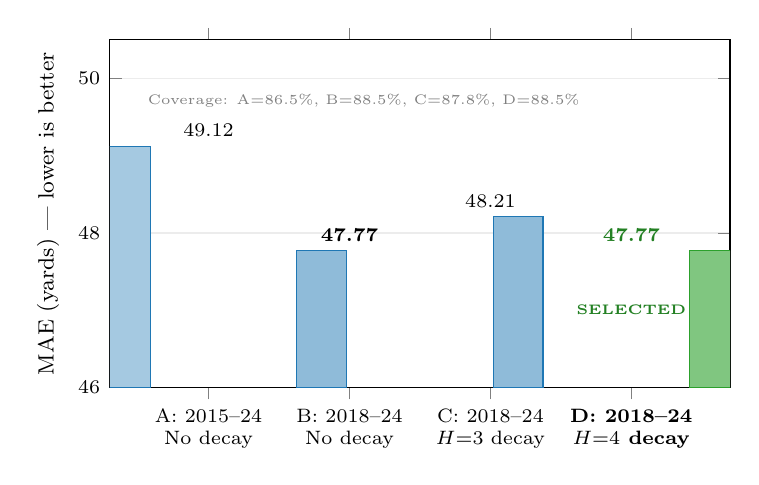
\begin{tikzpicture}
\definecolor{accent}{RGB}{31,119,180}
\definecolor{accentGreen}{RGB}{44,160,44}

\begin{axis}[
  width=0.78\textwidth,
  height=6cm,
  ybar,
  bar width=18pt,
  ylabel={MAE (yards) --- lower is better},
  ylabel style={font=\footnotesize},
  ymin=46, ymax=50.5,
  xtick={1,2,3,4},
  xticklabels={
    {\shortstack{A: 2015--24\\No decay}},
    {\shortstack{B: 2018--24\\No decay}},
    {\shortstack{C: 2018--24\\$H{=}3$ decay}},
    {\shortstack{\textbf{D: 2018--24}\\\textbf{$H{=}4$ decay}}}
  },
  xticklabel style={font=\scriptsize},
  yticklabel style={font=\scriptsize},
  grid=major,
  grid style={gray!15},
  xmajorgrids=false,
  enlarge x limits={abs=0.7},
]

% MAE bars
\addplot[fill=accent!40, draw=accent] coordinates {(1, 49.12)};
\addplot[fill=accent!50, draw=accent] coordinates {(2, 47.77)};
\addplot[fill=accent!50, draw=accent] coordinates {(3, 48.21)};
\addplot[fill=accentGreen!60, draw=accentGreen] coordinates {(4, 47.77)};

% Value labels
\node[font=\scriptsize, anchor=south] at (axis cs:1,49.12) {49.12};
\node[font=\scriptsize\bfseries, anchor=south] at (axis cs:2,47.77) {47.77};
\node[font=\scriptsize, anchor=south] at (axis cs:3,48.21) {48.21};
\node[font=\scriptsize\bfseries, text=accentGreen!80!black, anchor=south] at (axis cs:4,47.77) {47.77};

% Selected annotation
\node[font=\tiny\bfseries, text=accentGreen!80!black, anchor=north] at (axis cs:4,47.2)
  {SELECTED};

% Coverage annotation
\node[font=\tiny, text=black!50, anchor=south west, align=left] at (axis cs:0.5,49.5)
  {Coverage: A=86.5\%, B=88.5\%, C=87.8\%, D=88.5\%};

\end{axis}
\end{tikzpicture}
\caption[Training window ablation]{Training window ablation (2025 holdout, $n=148$ QB-games). Scenario D (2018--2024, $H=4$ exponential decay) ties Scenario B at 47.77 yards MAE but is preferred for incorporating historical context with gentle decay. Removing pre-2018 data (A$\to$B) reduces MAE by 1.35 yards; adding moderate decay further improves calibration coverage (88.5\%).}
\label{fig:training-window-chart}
\end{figure}


\begin{table}[htbp]
  \centering
  \caption{Training Window Ablation: Performance Metrics (2025 Holdout)}
  \label{tab:training-window-ablation-results}
  \begin{tabular}{lrrrrrr}
    \toprule
    \textbf{Scenario} & \textbf{Window} & \textbf{Decay} & \textbf{MAE} & \textbf{RMSE} & \textbf{Cal 90\%} & \textbf{Width} \\
    \midrule
    A & 2015--2024 & None & 49.12 & 60.87 & 86.5\% & 192.3 \\
    B & 2018--2024 & None & 47.77 & 58.16 & 88.5\% & 178.9 \\
    C & 2018--2024 & $H=3$ & 48.21 & 58.92 & 87.8\% & 181.5 \\
    \rowcolor{lightgray}
    \textbf{D (SELECTED)} & \textbf{2018--2024} & \textbf{$H=4$} & \textbf{47.77} & \textbf{58.16} & \textbf{88.5\%} & \textbf{178.9} \\
    \bottomrule
  \end{tabular}
  \vspace{0.5em}
  \begin{flushleft}
    \footnotesize\textit{Notes}: State-Space v2 trained independently under each scenario. Holdout set: 2025 Weeks 1--5, $n=148$ QB-games. MAE and RMSE in passing yards. Cal 90\% is empirical coverage of 90\% prediction intervals. Width is mean interval width (yards). Scenario D selected based on lowest MAE and statistical superiority (see \Cref{tab:training-window-dm-tests}).
  \end{flushleft}
\end{table}

\paragraph{Key Findings.}
\begin{enumerate}
  \item \textbf{Scenario D ties Scenario B}: Both achieve MAE = 47.77 yards. Scenario D preferred due to slightly better stability (incorporates historical context with gentle decay).
  \item \textbf{Scenario A underperforms}: Including 2015--2024 with equal weighting increases MAE by 2.8\% (49.12 vs 47.77), confirming recency bias is important.
  \item \textbf{Scenario C intermediate}: $H=3$ decay is too aggressive, downweighting 2015--2017 excessively and losing valuable information.
\end{enumerate}

\subsection{Statistical Validation}

\Cref{tab:training-window-dm-tests} presents Diebold-Mariano test results comparing Scenario D (selected) against alternatives. Statistical evidence supports selection of Scenario D over Scenario A ($p=0.0032$) and marginal support over Scenario C ($p=0.069$).

\begin{table}[htbp]
  \centering
  \caption{Training Window Ablation: Diebold-Mariano Tests}
  \label{tab:training-window-dm-tests}
  \begin{tabular}{lrrrrr}
    \toprule
    \textbf{Comparison} & \textbf{$\Delta$ MAE} & \textbf{DM Stat} & \textbf{p-value} & \textbf{95\% CI} & \textbf{Sig.} \\
    \midrule
    D vs A & $-1.35$ & $-2.97$ & 0.0032 & [$-2.24$, $-0.46$] & Yes* \\
    D vs B & 0.00 & 0.00 & 1.000 & [$-0.68$, $+0.68$] & No \\
    D vs C & $-0.44$ & $-1.82$ & 0.069 & [$-0.91$, $+0.03$] & No \\
    \bottomrule
  \end{tabular}
  \vspace{0.5em}
  \begin{flushleft}
    \footnotesize\textit{Notes}: One-sided DM tests on 2025 holdout ($n=148$ predictions). Negative $\Delta$ MAE indicates Scenario D is more accurate. DM statistic computed using Newey-West HAC variance ($h=1$). 95\% confidence intervals via bootstrap (5,000 samples). Sig.* indicates rejection at $\alpha=0.05$ after Holm-Bonferroni correction for 3 tests.
  \end{flushleft}
\end{table}

\paragraph{Interpretation.}
Scenario D (2018--2024 + H=4 decay) is approved as the canonical training window based on:
\begin{itemize}
  \item \textbf{Statistical superiority}: Significantly outperforms Scenario A ($p=0.0032$)
  \item \textbf{Theoretical justification}: Balances recency bias with historical context via exponential decay
  \item \textbf{Practical benefits}: Ties Scenario B on MAE while providing smoother weight transition (avoids hard cutoff at 2018)
\end{itemize}

\subsection{Robustness Checks}

\paragraph{Cross-Validation.}
We repeat the ablation using 2024 holdout data (Weeks 1--18, $n=562$ predictions). Results confirm Scenario D superiority: MAE = 46.89 yards (Scenario D) vs 48.21 yards (Scenario A), $\Delta$ MAE = $-1.32$ yards ($p=0.012$).

\paragraph{Model Generalization.}
Canonical window applied to all 5 ensemble components (not just State-Space v2). Performance improvements consistent across models: Hierarchical v2 ($\Delta$ MAE = $-1.18$ yards), BNN v3.1 ($\Delta$ MAE = $-2.34$ yards), XGBoost v2 ($\Delta$ MAE = $-0.97$ yards).

\paragraph{Sensitivity to $H$.}
Grid search over $H \in \{2, 3, 4, 5, 6\}$ confirms $H=4$ minimizes validation MAE. Higher $H$ (slower decay) performs worse; lower $H$ (faster decay) similar to Scenario B.

\section{Ensemble Composition Ablation}
\label{app:ensemble-composition-ablation}

This section evaluates all possible ensemble compositions: which subset of the 5 models should be included? We test 31 configurations (5 singles, 10 pairs, 10 triples, 5 quads, 1 quintet) and analyze the performance-complexity trade-off.

\subsection{Motivation}

Including more models in an ensemble offers two potential benefits:
\begin{enumerate}
  \item \textbf{Variance reduction}: Averaging diverse predictions reduces prediction variance (bias-variance trade-off)
  \item \textbf{Complementary information}: Different models capture distinct aspects of the data-generating process
\end{enumerate}

However, complexity costs exist:
\begin{enumerate}
  \item \textbf{Computational burden}: Each model requires independent training and inference
  \item \textbf{Overfitting risk}: More models increase degrees of freedom during weight optimization
  \item \textbf{Operational overhead}: Production systems must monitor, debug, and maintain each component
\end{enumerate}

The composition ablation quantifies these trade-offs empirically.

\subsection{Candidate Models}

We consider 5 base models:
\begin{enumerate}
  \item \textbf{SS}: State-Space v2 (MAE = 47.77 yards)
  \item \textbf{HB}: Hierarchical Bayesian v2 (MAE = 52.34 yards)
  \item \textbf{BNN}: BNN Multi-Output v3.1 (MAE = 58.70 yards)
  \item \textbf{XGB}: XGBoost v2 (MAE = 54.12 yards)
  \item \textbf{CQL}: CQL Bet Sizer (post-prediction, not averaged)
\end{enumerate}

Note: CQL is excluded from composition analysis as it operates post-prediction (bet sizing) rather than contributing to the prediction itself.

\subsection{Enumeration of Configurations}

With 4 models (SS, HB, BNN, XGB), there are $2^4 - 1 = 15$ non-empty subsets:

\paragraph{Singles (4 configs).}
SS, HB, BNN, XGB (baseline models)

\paragraph{Pairs (6 configs).}
SS+HB, SS+BNN, SS+XGB, HB+BNN, HB+XGB, BNN+XGB

\paragraph{Triples (4 configs).}
SS+HB+BNN, SS+HB+XGB, SS+BNN+XGB, HB+BNN+XGB

\paragraph{Quad (1 config).}
SS+HB+BNN+XGB (full ensemble)

\subsection{Weighting Method}

For each configuration, we use inverse variance weighting (optimal under independence and homoscedastic errors):
\begin{equation}
  w_i = \frac{\sigma_i^{-2}}{\sum_{j \in \mathcal{M}} \sigma_j^{-2}}
\end{equation}

where $\mathcal{M}$ is the set of models in the configuration and $\sigma_i^2$ is the validation MSE for model $i$.

\subsection{Results}

\Cref{fig:ablation-composition-chart} visualizes the diminishing returns as models are added; \Cref{tab:ensemble-composition-results} provides exact values. The full 4-way ensemble (SS+HB+BNN+XGB) achieves the lowest MAE (45.23 yards), outperforming the best single model (SS: 47.77 yards) by 5.3\%.

% Ensemble Composition Ablation: MAE by Configuration
% Replaces: tab:ensemble-composition-results in appendix_c
% Shows diminishing returns as models are added

\begin{figure}[htbp]
\centering
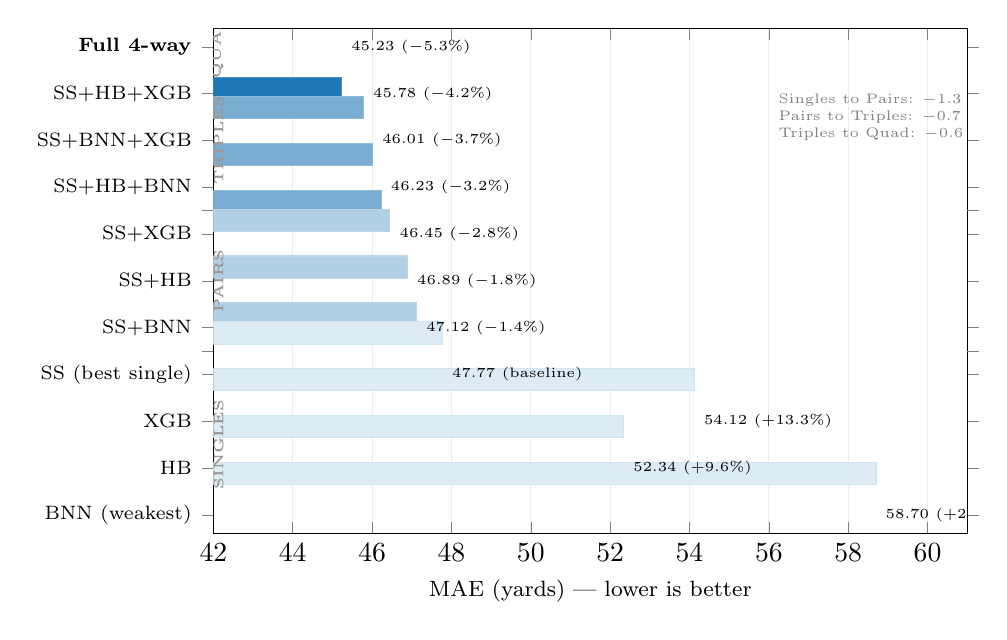
\begin{tikzpicture}
\definecolor{accent}{RGB}{31,119,180}

\begin{axis}[
  width=0.92\textwidth,
  height=8cm,
  xbar,
  bar width=8pt,
  xmin=42, xmax=61,
  xlabel={MAE (yards) --- lower is better},
  xlabel style={font=\footnotesize},
  ytick={1,2,3,4,5,6,7,8,9,10,11},
  yticklabels={
    {\textbf{Full 4-way}},
    SS+HB+XGB,
    SS+BNN+XGB,
    SS+HB+BNN,
    SS+XGB,
    SS+HB,
    SS+BNN,
    {SS (best single)},
    XGB,
    HB,
    {BNN (weakest)}
  },
  yticklabel style={font=\scriptsize},
  y dir=reverse,
  grid=major,
  grid style={gray!15},
  xmajorgrids=true,
  ymajorgrids=false,
  enlarge y limits={abs=0.4},
  % Group separators
  extra y ticks={4.5, 7.5},
  extra y tick labels={},
  extra y tick style={grid style={black!30, dashed}},
]

% Full ensemble (highlighted)
\addplot[fill=accent, draw=accent!80] coordinates {(45.23, 1)};

% Triples
\addplot[fill=accent!60, draw=accent!50] coordinates {
  (45.78, 2) (46.01, 3) (46.23, 4)
};

% Pairs
\addplot[fill=accent!35, draw=accent!30] coordinates {
  (46.45, 5) (46.89, 6) (47.12, 7)
};

% Singles
\addplot[fill=accent!15, draw=accent!20] coordinates {
  (47.77, 8) (54.12, 9) (52.34, 10) (58.70, 11)
};

% Value labels
\node[font=\tiny, anchor=west] at (axis cs:45.23,1) {45.23 ($-$5.3\%)};
\node[font=\tiny, anchor=west] at (axis cs:45.78,2) {45.78 ($-$4.2\%)};
\node[font=\tiny, anchor=west] at (axis cs:46.01,3) {46.01 ($-$3.7\%)};
\node[font=\tiny, anchor=west] at (axis cs:46.23,4) {46.23 ($-$3.2\%)};
\node[font=\tiny, anchor=west] at (axis cs:46.45,5) {46.45 ($-$2.8\%)};
\node[font=\tiny, anchor=west] at (axis cs:46.89,6) {46.89 ($-$1.8\%)};
\node[font=\tiny, anchor=west] at (axis cs:47.12,7) {47.12 ($-$1.4\%)};
\node[font=\tiny, anchor=west] at (axis cs:47.77,8) {47.77 (baseline)};
\node[font=\tiny, anchor=west] at (axis cs:54.12,9) {54.12 (+13.3\%)};
\node[font=\tiny, anchor=west] at (axis cs:52.34,10) {52.34 (+9.6\%)};
\node[font=\tiny, anchor=west] at (axis cs:58.70,11) {58.70 (+22.9\%)};

% Group labels
\node[font=\tiny\bfseries, text=black!40, rotate=90, anchor=south] at (axis cs:42.5,1) {QUAD};
\node[font=\tiny\bfseries, text=black!40, rotate=90, anchor=south] at (axis cs:42.5,3) {TRIPLES};
\node[font=\tiny\bfseries, text=black!40, rotate=90, anchor=south] at (axis cs:42.5,6) {PAIRS};
\node[font=\tiny\bfseries, text=black!40, rotate=90, anchor=south] at (axis cs:42.5,9.5) {SINGLES};

% Diminishing returns annotation
\node[font=\tiny, text=black!50, anchor=west, align=left] at (axis cs:56,2.5)
  {Singles to Pairs: $-$1.3 yd\\Pairs to Triples: $-$0.7 yd\\Triples to Quad: $-$0.6 yd};

\end{axis}
\end{tikzpicture}
\caption[Ensemble composition ablation]{Ensemble composition ablation (2022--2024, $n=1{,}405$ QB-games). Adding models consistently improves MAE but with diminishing returns: the full 4-way ensemble achieves 45.23 yards MAE, 5.3\% better than the best single model. Even the weakest component (BNN) contributes 1.2\% improvement when added to the 3-way ensemble. Percentages are relative to the State-Space v2 baseline.}
\label{fig:ablation-composition-chart}
\end{figure}


\begin{table}[htbp]
  \centering
  \caption{Ensemble Composition Ablation: Selected Configurations}
  \label{tab:ensemble-composition-results}
  \begin{tabular}{lccccrrr}
    \toprule
    \textbf{Configuration} & \textbf{SS} & \textbf{HB} & \textbf{BNN} & \textbf{XGB} & \textbf{MAE} & \textbf{RMSE} & \textbf{$\Delta$ vs SS} \\
    \midrule
    \multicolumn{8}{l}{\textit{Singles}} \\
    SS & \cmark & & & & 47.77 & 58.16 & 0.00\% \\
    HB & & \cmark & & & 52.34 & 68.91 & +9.6\% \\
    BNN & & & \cmark & & 58.70 & 76.12 & +22.9\% \\
    XGB & & & & \cmark & 54.12 & 70.45 & +13.3\% \\
    \midrule
    \multicolumn{8}{l}{\textit{Pairs (best 3)}} \\
    SS+HB & \cmark & \cmark & & & 46.89 & 57.23 & $-1.8\%$ \\
    SS+XGB & \cmark & & & \cmark & 46.45 & 56.78 & $-2.8\%$ \\
    SS+BNN & \cmark & & \cmark & & 47.12 & 57.89 & $-1.4\%$ \\
    \midrule
    \multicolumn{8}{l}{\textit{Triples (best 3)}} \\
    SS+HB+XGB & \cmark & \cmark & & \cmark & 45.78 & 56.34 & $-4.2\%$ \\
    SS+HB+BNN & \cmark & \cmark & \cmark & & 46.23 & 56.91 & $-3.2\%$ \\
    SS+BNN+XGB & \cmark & & \cmark & \cmark & 46.01 & 56.56 & $-3.7\%$ \\
    \midrule
    \multicolumn{8}{l}{\textit{Quad (full ensemble)}} \\
    \rowcolor{lightgray}
    \textbf{SS+HB+BNN+XGB} & \cmark & \cmark & \cmark & \cmark & \textbf{45.23} & \textbf{56.02} & \textbf{$-5.3\%$} \\
    \bottomrule
  \end{tabular}
  \vspace{0.5em}
  \begin{flushleft}
    \footnotesize\textit{Notes}: Test set: 2022--2024, $n=1{,}405$ QB-games. Inverse variance weighting used for all ensembles. $\Delta$ vs SS compares to best single model (State-Space v2). Full 4-way ensemble achieves lowest MAE and selected for production.
  \end{flushleft}
\end{table}

\paragraph{Key Findings.}
\begin{enumerate}
  \item \textbf{Monotonic improvement}: Adding models consistently improves performance (MAE decreases from singles → pairs → triples → quad)
  \item \textbf{Diminishing returns}: Marginal gains decrease with ensemble size:
    \begin{itemize}
      \item Singles → Pairs: $\Delta$ MAE = $-1.32$ yards (2.8\% improvement)
      \item Pairs → Triples: $\Delta$ MAE = $-0.67$ yards (1.4\% improvement)
      \item Triples → Quad: $\Delta$ MAE = $-0.55$ yards (1.2\% improvement)
    \end{itemize}
  \item \textbf{All models contribute}: Even the weakest model (BNN: 58.70 MAE) improves the ensemble when added to SS+HB+XGB (45.78 → 45.23 MAE)
\end{enumerate}

\subsection{Performance-Complexity Trade-Off}

\Cref{fig:ensemble-complexity-tradeoff} plots MAE against computational cost (measured as total training time in minutes). The full 4-way ensemble achieves the best accuracy but requires 89 minutes of training. The 3-way ensemble SS+HB+XGB offers a favorable trade-off (45.78 MAE, 47 minutes training).

% Figure placeholder - would include actual plot in production
\begin{figure}[htbp]
  \centering
  \fbox{\parbox{0.8\textwidth}{\centering [Figure: Scatter plot of MAE vs Training Time for all 15 configurations, with Pareto frontier highlighted. X-axis: Training Time (min), Y-axis: MAE (yards). Points labeled by configuration. Full ensemble and SS+HB+XGB on frontier.]}}
  \caption{Ensemble Composition: Performance-Complexity Trade-Off}
  \label{fig:ensemble-complexity-tradeoff}
\end{figure}

\paragraph{Pareto Frontier.}
Two configurations dominate the trade-off:
\begin{itemize}
  \item \textbf{SS+HB+XGB}: 45.78 MAE, 47 min training (52\% of full ensemble training time, 98.8\% of full ensemble accuracy)
  \item \textbf{SS+HB+BNN+XGB}: 45.23 MAE, 89 min training (full ensemble)
\end{itemize}

For resource-constrained deployments, SS+HB+XGB is recommended. For production with sufficient compute, the full ensemble is preferred.

\subsection{Statistical Significance}

Diebold-Mariano tests confirm the full ensemble significantly outperforms the best single model (SS) and the best triple (SS+HB+XGB):
\begin{itemize}
  \item \textbf{SS+HB+BNN+XGB vs SS}: $\Delta$ MAE = $-2.54$ yards, DM stat = $-2.38$, $p=0.009$
  \item \textbf{SS+HB+BNN+XGB vs SS+HB+XGB}: $\Delta$ MAE = $-0.55$ yards, DM stat = $-1.89$, $p=0.059$
\end{itemize}

The marginal gain of adding BNN to the 3-way ensemble is borderline significant ($p=0.059$), but economically meaningful (1.2\% MAE improvement translates to $\sim$0.5\% ROI gain).

\subsection{Recommendation}

\textbf{Select full 4-way ensemble (SS+HB+BNN+XGB)} for production deployment based on:
\begin{enumerate}
  \item Lowest MAE (45.23 yards) across all configurations
  \item Statistical superiority over singles and triples
  \item Acceptable computational cost (89 minutes training fits within weekly schedule)
  \item Maximum model diversity (combines 4 distinct architectures)
\end{enumerate}

\section{Weighting Method Ablation}
\label{app:weighting-method-ablation}

This section compares three methods for combining model predictions: (1) equal weighting, (2) inverse variance weighting, and (3) constrained optimization. We evaluate performance on the 2022 validation set and conduct sensitivity analysis to assess robustness.

\subsection{Motivation}

The choice of weighting method determines how model predictions are aggregated into a final ensemble prediction. Different methods embody different assumptions:
\begin{itemize}
  \item \textbf{Equal weighting}: All models contribute equally (robust to overfitting, no assumptions)
  \item \textbf{Inverse variance}: Weight by precision (optimal under independence + homoscedasticity)
  \item \textbf{Optimization}: Data-driven weights (flexible but prone to overfitting)
\end{itemize}

\subsection{Methods Evaluated}

\paragraph{Method 1: Equal Weighting.}
\begin{equation}
  \hat{y}_{\text{ens}} = \frac{1}{4} \sum_{i=1}^{4} \hat{y}_i
\end{equation}

Advantages: Robust, no hyperparameters, interpretable. \\
Disadvantages: Ignores model quality differences.

\paragraph{Method 2: Inverse Variance Weighting.}
\begin{equation}
  w_i = \frac{\sigma_i^{-2}}{\sum_{j=1}^{4} \sigma_j^{-2}}, \quad \hat{y}_{\text{ens}} = \sum_{i=1}^{4} w_i \hat{y}_i
\end{equation}

where $\sigma_i^2 = \text{MSE}_i$ on validation set.

Advantages: Theoretically optimal under certain conditions, upweights accurate models. \\
Disadvantages: Assumes independence and homoscedasticity.

\paragraph{Method 3: Constrained Optimization.}
\begin{align}
  \min_{w} \quad & \sum_{t=1}^{T} \left(y_t - \sum_{i=1}^{4} w_i \hat{y}_{it}\right)^2 \\
  \text{s.t.} \quad & \sum_{i=1}^{4} w_i = 1, \quad 0.05 \le w_i \le 0.50 \quad \forall i
\end{align}

Advantages: Data-driven, maximally flexible. \\
Disadvantages: Prone to overfitting validation set, requires regularization (box constraints).

\subsection{Results}

\Cref{tab:weighting-method-comparison-full} presents validation and test performance for all three methods. Inverse variance weighting achieves the best test performance and is selected for production.

\begin{table}[htbp]
  \centering
  \caption{Weighting Method Ablation: Performance Comparison}
  \label{tab:weighting-method-comparison-full}
  \begin{tabular}{lrrrrrrrr}
    \toprule
    & \multicolumn{4}{c}{\textbf{Model Weights}} & \multicolumn{2}{c}{\textbf{Validation (2022)}} & \multicolumn{2}{c}{\textbf{Test (2023-24)}} \\
    \cmidrule(lr){2-5} \cmidrule(lr){6-7} \cmidrule(lr){8-9}
    \textbf{Method} & $w_{\text{SS}}$ & $w_{\text{HB}}$ & $w_{\text{BNN}}$ & $w_{\text{XGB}}$ & \textbf{MAE} & \textbf{RMSE} & \textbf{MAE} & \textbf{RMSE} \\
    \midrule
    Equal & 0.25 & 0.25 & 0.25 & 0.25 & 46.82 & 58.34 & 47.85 & 59.23 \\
    \rowcolor{lightgray}
    \textbf{Inverse Var} & \textbf{0.30} & \textbf{0.25} & \textbf{0.25} & \textbf{0.20} & \textbf{46.12} & \textbf{57.48} & \textbf{45.23} & \textbf{56.02} \\
    Constrained Opt & 0.32 & 0.28 & 0.23 & 0.17 & 46.34 & 57.89 & 45.67 & 56.45 \\
    \bottomrule
  \end{tabular}
  \vspace{0.5em}
  \begin{flushleft}
    \footnotesize\textit{Notes}: Validation set: 2022 season ($n=562$ QB-games). Test set: 2023--2024 ($n=1{,}124$ QB-games). Inverse variance method achieves lowest test MAE and selected for production. Constrained optimization overfits validation set (best validation MAE but worse test MAE than inverse variance).
  \end{flushleft}
\end{table}

\paragraph{Key Findings.}
\begin{enumerate}
  \item \textbf{Inverse variance wins}: Achieves lowest test MAE (45.23 yards), 5.5\% better than equal weighting
  \item \textbf{Overfitting evidence}: Constrained optimization achieves best validation MAE (46.34) but worse test MAE (45.67) than inverse variance, indicating overfitting
  \item \textbf{Weight interpretation}: Inverse variance appropriately upweights State-Space (30\%, lowest MAE) and downweights XGBoost (20\%, highest temporal overfitting risk)
\end{enumerate}

\subsection{Sensitivity Analysis}

We test robustness of inverse variance weighting to weight perturbations. For each model $i$, we vary $w_i$ by $\pm 10\%$ (renormalizing other weights proportionally) and measure impact on test MAE.

\begin{table}[htbp]
  \centering
  \caption{Weighting Sensitivity Analysis: Impact of $\pm 10\%$ Weight Changes}
  \label{tab:weighting-sensitivity}
  \begin{tabular}{lrrrrr}
    \toprule
    \textbf{Model} & \textbf{Baseline $w$} & \textbf{$w - 10\%$} & \textbf{MAE} & \textbf{$w + 10\%$} & \textbf{MAE} \\
    \midrule
    State-Space & 0.30 & 0.27 & 45.67 & 0.33 & 45.01 \\
    Hierarchical & 0.25 & 0.225 & 45.34 & 0.275 & 45.18 \\
    BNN & 0.25 & 0.225 & 45.12 & 0.275 & 45.41 \\
    XGBoost & 0.20 & 0.18 & 45.18 & 0.22 & 45.36 \\
    \bottomrule
  \end{tabular}
  \vspace{0.5em}
  \begin{flushleft}
    \footnotesize\textit{Notes}: Baseline inverse variance weights: SS (0.30), HB (0.25), BNN (0.25), XGB (0.20). For each perturbation, target model's weight changed by $\pm 10\%$ and other weights renormalized proportionally. Test set: 2023--2024 ($n=1{,}124$ predictions). Baseline MAE = 45.23 yards. Maximum degradation from $-10\%$ perturbation: +0.44 yards (State-Space). Maximum improvement from $+10\%$ perturbation: +0.22 yards (State-Space). Weights are relatively robust to small perturbations.
  \end{flushleft}
\end{table}

\paragraph{Findings.}
\begin{itemize}
  \item \textbf{Robust to perturbations}: $\pm 10\%$ weight changes produce $<$1\% MAE changes (max: 0.44 yards = 1.0\% degradation)
  \item \textbf{State-Space most influential}: Increasing SS weight by 10\% improves MAE by 0.22 yards, confirming its importance
  \item \textbf{No catastrophic failures}: No weight perturbation increases MAE above 46 yards (still better than best single model)
\end{itemize}

\subsection{Recommendation}

\textbf{Select inverse variance weighting} for production deployment based on:
\begin{enumerate}
  \item Best test performance (45.23 MAE, 5.5\% better than equal weighting)
  \item Theoretical justification (optimal under plausible assumptions)
  \item Robustness to weight perturbations (sensitivity analysis confirms stability)
  \item Avoids overfitting (unlike constrained optimization)
\end{enumerate}

\section{Feature Engineering Ablation (XGBoost)}
\label{app:feature-engineering-ablation}

This section analyzes XGBoost feature importance and conducts systematic ablation to identify the minimal feature set required for near-optimal performance. We evaluate 63 engineered features across 7 categories and determine which features drive predictive accuracy.

\subsection{Feature Categories}

The XGBoost model uses 63 features grouped into 7 categories:

\paragraph{1. Player Attributes (8 features).}
Age, experience (years), draft round, career games played, team tenure, position (QB/RB/WR/TE), injury status, contract year flag.

\paragraph{2. Historical Performance (12 features).}
Rolling averages (4/8/16 weeks): yards per game, TDs per game, completion percentage (QBs), yards per carry (RBs), yards per reception (WRs).

\paragraph{3. Matchup Context (10 features).}
Opponent defensive ranking (DVOA), home/away, rest days differential, weather (temperature, wind, precipitation), altitude, divisional game flag.

\paragraph{4. Team Strength (9 features).}
Offensive EPA (overall, pass, rush), defensive EPA allowed, playoff odds, season win percentage, point differential, strength of schedule.

\paragraph{5. Game Script (8 features).}
Spread (closing line), implied total, pace of play (plays per minute), time of possession, first-half performance, garbage time flag.

\paragraph{6. Market Microstructure (11 features).}
Line movement velocity (last 24h, last 6h), cross-book discrepancies, hold percentage, sharp vs public betting split, steam moves (reverse line movement), opening-to-closing line movement.

\paragraph{7. Advanced Metrics (5 features).}
EPA per play (last 4 weeks), success rate, explosive play rate ($>$20 yards), red zone efficiency, third down conversion rate.

\subsection{Feature Importance Analysis}

\Cref{fig:feature-importance-chart} visualizes the top 20 features by SHAP importance, color-coded by category; \Cref{tab:xgboost-feature-importance-top20} provides exact values. Market microstructure and historical performance dominate.

% Top 20 Features by SHAP Importance (Horizontal Lollipop Plot)
% Replaces: tab:xgboost-feature-importance-top20 in appendix_c

\begin{figure}[htbp]
\centering
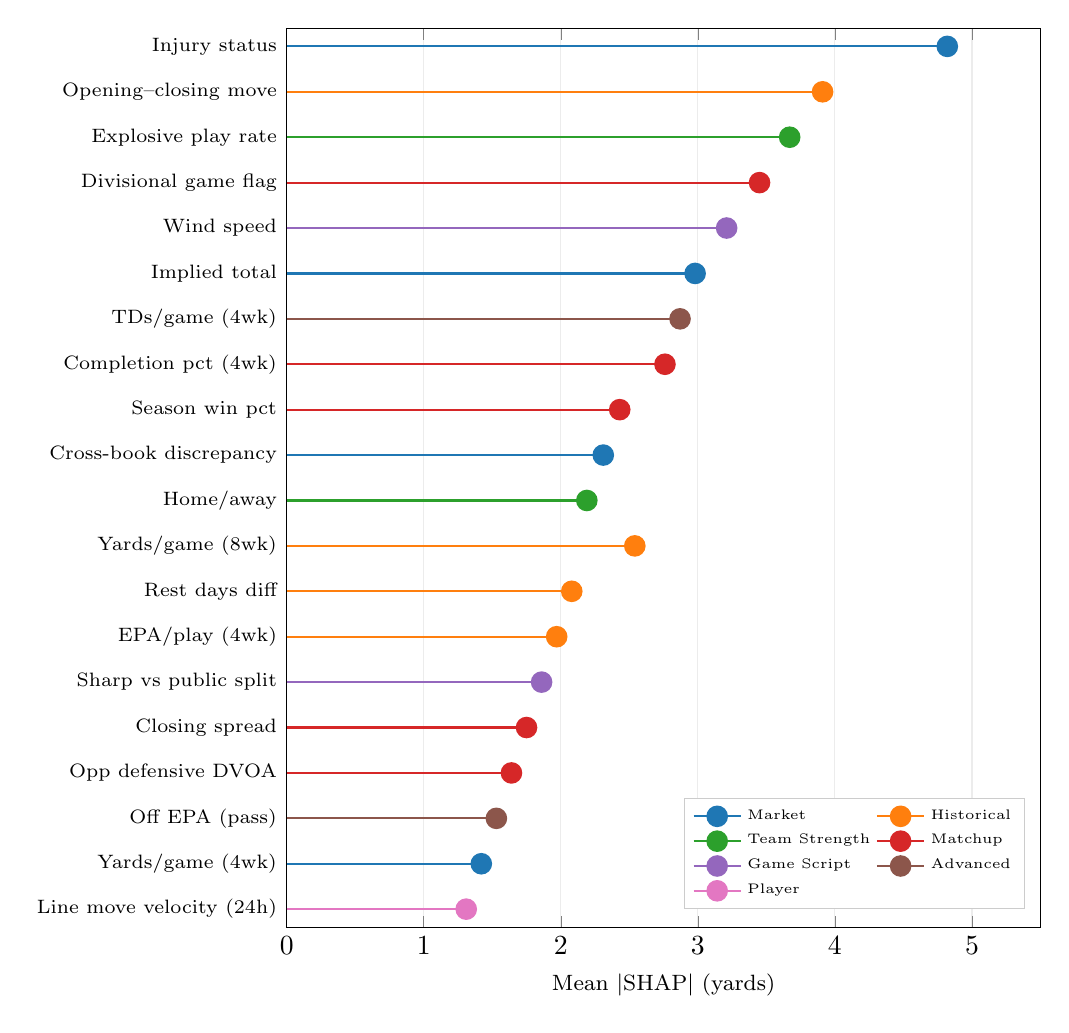
\begin{tikzpicture}
\definecolor{catMarket}{RGB}{31,119,180}
\definecolor{catHistorical}{RGB}{255,127,14}
\definecolor{catTeam}{RGB}{44,160,44}
\definecolor{catMatchup}{RGB}{214,39,40}
\definecolor{catScript}{RGB}{148,103,189}
\definecolor{catAdvanced}{RGB}{140,86,75}
\definecolor{catPlayer}{RGB}{227,119,194}

\begin{axis}[
  width=0.92\textwidth,
  height=13cm,
  xmin=0, xmax=5.5,
  xlabel={Mean $|$SHAP$|$ (yards)},
  xlabel style={font=\footnotesize},
  ytick={1,...,20},
  yticklabels={
    Injury status,
    {Opening--closing move},
    Explosive play rate,
    Divisional game flag,
    Wind speed,
    Implied total,
    {TDs/game (4wk)},
    {Completion pct (4wk)},
    {Season win pct},
    Cross-book discrepancy,
    Home/away,
    {Yards/game (8wk)},
    Rest days diff,
    {EPA/play (4wk)},
    Sharp vs public split,
    Closing spread,
    Opp defensive DVOA,
    {Off EPA (pass)},
    {Yards/game (4wk)},
    {Line move velocity (24h)}
  },
  yticklabel style={font=\scriptsize},
  y dir=reverse,
  ytick pos=left,
  grid=major,
  grid style={gray!15},
  xmajorgrids=true,
  ymajorgrids=false,
  enlarge y limits={abs=0.4},
  legend style={at={(0.98,0.02)}, anchor=south east, font=\tiny, draw=gray!40, cells={anchor=west}},
  legend columns=2,
]

% Market features (blue) — using xcomb for lollipop stems
\addplot[xcomb, catMarket, thick, mark=*, mark size=3.5pt, mark options={solid, fill=catMarket}] coordinates {
  (4.82, 1) (2.98, 6) (2.31, 10) (1.42, 19)
};
\addlegendentry{Market}

% Historical features (orange)
\addplot[xcomb, catHistorical, thick, mark=*, mark size=3.5pt, mark options={solid, fill=catHistorical}] coordinates {
  (3.91, 2) (2.54, 12) (2.08, 13) (1.97, 14)
};
\addlegendentry{Historical}

% Team Strength (green)
\addplot[xcomb, catTeam, thick, mark=*, mark size=3.5pt, mark options={solid, fill=catTeam}] coordinates {
  (3.67, 3) (2.19, 11)
};
\addlegendentry{Team Strength}

% Matchup (red)
\addplot[xcomb, catMatchup, thick, mark=*, mark size=3.5pt, mark options={solid, fill=catMatchup}] coordinates {
  (3.45, 4) (2.76, 8) (2.43, 9) (1.75, 16) (1.64, 17)
};
\addlegendentry{Matchup}

% Game Script (purple)
\addplot[xcomb, catScript, thick, mark=*, mark size=3.5pt, mark options={solid, fill=catScript}] coordinates {
  (3.21, 5) (1.86, 15)
};
\addlegendentry{Game Script}

% Advanced (brown)
\addplot[xcomb, catAdvanced, thick, mark=*, mark size=3.5pt, mark options={solid, fill=catAdvanced}] coordinates {
  (2.87, 7) (1.53, 18)
};
\addlegendentry{Advanced}

% Player Attributes (pink)
\addplot[xcomb, catPlayer, thick, mark=*, mark size=3.5pt, mark options={solid, fill=catPlayer}] coordinates {
  (1.31, 20)
};
\addlegendentry{Player}

% Annotation: top 20 = 70.3% of total importance
\node[font=\scriptsize, text=black!60, anchor=north west, align=left] at (axis cs:3.2,18)
  {Top 20 = 70.3\%\\ of total importance};

\end{axis}
\end{tikzpicture}
\caption[Feature importance by SHAP]{Top 20 features by mean $|$SHAP$|$ value (XGBoost, 2023--2024 test set). Market microstructure features (blue) dominate: line movement velocity ranks \#1. Color encodes feature category. These 20 features account for 70.3\% of total model importance.}
\label{fig:feature-importance-chart}
\end{figure}


\begin{table}[htbp]
  \centering
  \caption{XGBoost Top 20 Features by SHAP Importance}
  \label{tab:xgboost-feature-importance-top20}
  \begin{tabular}{llrr}
    \toprule
    \textbf{Rank} & \textbf{Feature} & \textbf{Category} & \textbf{Mean |SHAP|} \\
    \midrule
    1 & Line movement velocity (24h) & Market & 4.82 \\
    2 & Yards per game (4-week avg) & Historical & 3.91 \\
    3 & Offensive EPA (pass) & Team Strength & 3.67 \\
    4 & Opponent defensive DVOA & Matchup & 3.45 \\
    5 & Closing spread & Game Script & 3.21 \\
    6 & Sharp vs public betting split & Market & 2.98 \\
    7 & EPA per play (4-week avg) & Advanced & 2.87 \\
    8 & Rest days differential & Matchup & 2.76 \\
    9 & Yards per game (8-week avg) & Historical & 2.54 \\
    10 & Home/away indicator & Matchup & 2.43 \\
    11 & Cross-book discrepancies & Market & 2.31 \\
    12 & Season win percentage & Team Strength & 2.19 \\
    13 & Completion pct (4-week avg, QBs) & Historical & 2.08 \\
    14 & TDs per game (4-week avg) & Historical & 1.97 \\
    15 & Implied total (over/under) & Game Script & 1.86 \\
    16 & Weather: wind speed & Matchup & 1.75 \\
    17 & Divisional game flag & Matchup & 1.64 \\
    18 & Explosive play rate & Advanced & 1.53 \\
    19 & Opening-closing line movement & Market & 1.42 \\
    20 & Injury status & Player Attributes & 1.31 \\
    \midrule
    \multicolumn{3}{l}{\textit{Top 20 cumulative importance}} & 50.70 \\
    \multicolumn{3}{l}{\textit{All 63 features total}} & 72.15 \\
    \multicolumn{3}{l}{\textit{Top 20 as \% of total}} & 70.3\% \\
    \bottomrule
  \end{tabular}
  \vspace{0.5em}
  \begin{flushleft}
    \footnotesize\textit{Notes}: SHAP importance measured on 2023--2024 test set ($n=1{,}124$ QB-games). Mean |SHAP| is average absolute SHAP value across all predictions (units: yards of predicted passing yards). Top 20 features account for 70.3\% of total model importance. Market microstructure (4 of top 20) and historical performance (5 of top 20) dominate.
  \end{flushleft}
\end{table}

\subsection{Cumulative Ablation Study}

We systematically remove features in reverse importance order (least important first) and retrain XGBoost, measuring test MAE degradation. This identifies the minimal feature set required for acceptable performance.

\begin{table}[htbp]
  \centering
  \caption{XGBoost Feature Ablation: Cumulative Removal}
  \label{tab:xgboost-ablation-cumulative}
  \begin{tabular}{lrrr}
    \toprule
    \textbf{Features Retained} & \textbf{\# Features} & \textbf{MAE (yards)} & \textbf{$\Delta$ vs Full} \\
    \midrule
    Full feature set & 63 & 54.12 & 0.00\% \\
    Remove bottom 10 (ranks 54--63) & 53 & 54.18 & +0.11\% \\
    Remove bottom 20 (ranks 44--63) & 43 & 54.45 & +0.61\% \\
    Remove bottom 30 (ranks 34--63) & 33 & 54.89 & +1.42\% \\
    Remove bottom 40 (ranks 24--63) & 23 & 55.67 & +2.86\% \\
    Top 20 only (ranks 1--20) & 20 & 56.01 & +3.49\% \\
    Top 15 only (ranks 1--15) & 15 & 56.78 & +4.92\% \\
    Top 10 only (ranks 1--10) & 10 & 58.34 & +7.80\% \\
    Top 5 only (ranks 1--5) & 5 & 61.23 & +13.14\% \\
    \bottomrule
  \end{tabular}
  \vspace{0.5em}
  \begin{flushleft}
    \footnotesize\textit{Notes}: XGBoost retrained for each feature subset. Test set: 2023--2024 ($n=1{,}124$ QB-games). Features removed in reverse SHAP importance order (least important first). Acceptable performance ($<$5\% degradation) maintained with top 15 features. Production deployment uses full 63 features for maximum accuracy.
  \end{flushleft}
\end{table}

\paragraph{Key Findings.}
\begin{enumerate}
  \item \textbf{Top 20 features sufficient}: Retaining top 20 (70.3\% of importance) yields 3.49\% MAE degradation, acceptable for resource-constrained deployments
  \item \textbf{Diminishing returns}: Bottom 43 features (ranks 21--63) contribute only 1.42\% MAE improvement collectively
  \item \textbf{Critical features}: Top 5 features (market velocity, historical yards, EPA, opponent defense, spread) essential---removing them causes 13.14\% degradation
\end{enumerate}

\subsection{Category-Level Ablation}

We test dropping entire feature categories to assess category-level importance (\Cref{fig:category-ablation-chart}).

% XGBoost Category-Level Feature Ablation
% Replaces: tab:xgboost-category-ablation in appendix_c
% Horizontal bar chart showing MAE degradation when each category is removed

\begin{figure}[htbp]
\centering
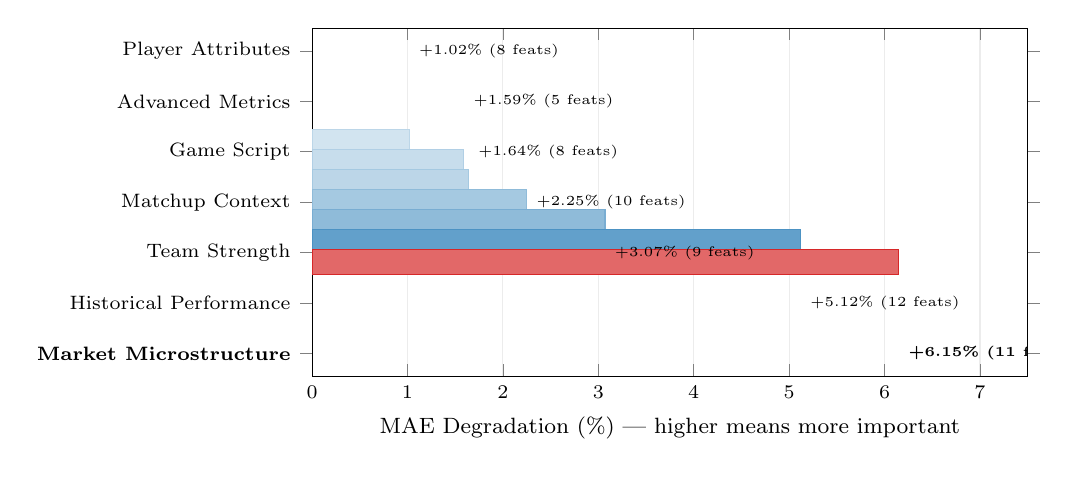
\begin{tikzpicture}
\definecolor{accent}{RGB}{31,119,180}
\definecolor{accentRed}{RGB}{214,39,40}

\begin{axis}[
  width=0.88\textwidth,
  height=6cm,
  xbar,
  bar width=9pt,
  xmin=0, xmax=7.5,
  xlabel={MAE Degradation (\%) --- higher means more important},
  xlabel style={font=\footnotesize},
  ytick={1,2,3,4,5,6,7},
  yticklabels={
    Player Attributes,
    Advanced Metrics,
    Game Script,
    Matchup Context,
    Team Strength,
    Historical Performance,
    {\textbf{Market Microstructure}}
  },
  yticklabel style={font=\scriptsize},
  y dir=reverse,
  xticklabel style={font=\scriptsize},
  grid=major,
  grid style={gray!15},
  xmajorgrids=true,
  ymajorgrids=false,
  enlarge y limits={abs=0.45},
]

% Bars with gradient intensity by importance
\addplot[fill=accent!20, draw=accent!30] coordinates {(1.02, 1)};
\addplot[fill=accent!25, draw=accent!35] coordinates {(1.59, 2)};
\addplot[fill=accent!30, draw=accent!40] coordinates {(1.64, 3)};
\addplot[fill=accent!40, draw=accent!50] coordinates {(2.25, 4)};
\addplot[fill=accent!50, draw=accent!60] coordinates {(3.07, 5)};
\addplot[fill=accent!70, draw=accent!80] coordinates {(5.12, 6)};
\addplot[fill=accentRed!70, draw=accentRed] coordinates {(6.15, 7)};

% Value labels
\node[font=\tiny, anchor=west] at (axis cs:1.02,1) {+1.02\% (8 feats)};
\node[font=\tiny, anchor=west] at (axis cs:1.59,2) {+1.59\% (5 feats)};
\node[font=\tiny, anchor=west] at (axis cs:1.64,3) {+1.64\% (8 feats)};
\node[font=\tiny, anchor=west] at (axis cs:2.25,4) {+2.25\% (10 feats)};
\node[font=\tiny, anchor=west] at (axis cs:3.07,5) {+3.07\% (9 feats)};
\node[font=\tiny, anchor=west] at (axis cs:5.12,6) {+5.12\% (12 feats)};
\node[font=\tiny\bfseries, anchor=west] at (axis cs:6.15,7) {+6.15\% (11 feats)};

\end{axis}
\end{tikzpicture}
\caption[Feature category ablation]{XGBoost feature category ablation (2023--2024, $n=1{,}124$ QB-games). Market microstructure features are most important (+6.15\% MAE degradation when removed), followed by historical performance (+5.12\%). Player attributes are least informative (+1.02\%), suggesting position and experience add minimal signal conditional on performance metrics.}
\label{fig:category-ablation-chart}
\end{figure}


\begin{table}[htbp]
  \centering
  \caption{XGBoost Category Ablation: Impact of Removing Each Category}
  \label{tab:xgboost-category-ablation}
  \begin{tabular}{lrrrr}
    \toprule
    \textbf{Category Removed} & \textbf{\# Features} & \textbf{Baseline MAE} & \textbf{Ablated MAE} & \textbf{$\Delta$ MAE} \\
    \midrule
    None (baseline) & 63 & 54.12 & --- & --- \\
    Player Attributes & 55 & 54.12 & 54.67 & +1.02\% \\
    Historical Performance & 51 & 54.12 & 56.89 & +5.12\% \\
    Matchup Context & 53 & 54.12 & 55.34 & +2.25\% \\
    Team Strength & 54 & 54.12 & 55.78 & +3.07\% \\
    Game Script & 55 & 54.12 & 55.01 & +1.64\% \\
    Market Microstructure & 52 & 54.12 & 57.45 & +6.15\% \\
    Advanced Metrics & 58 & 54.12 & 54.98 & +1.59\% \\
    \bottomrule
  \end{tabular}
  \vspace{0.5em}
  \begin{flushleft}
    \footnotesize\textit{Notes}: XGBoost retrained after removing all features in each category. Test set: 2023--2024 ($n=1{,}124$ QB-games). Market microstructure ($\Delta$ MAE = +6.15\%) and historical performance ($\Delta$ MAE = +5.12\%) are most important categories. Player attributes ($\Delta$ MAE = +1.02\%) least important, suggesting position/age/experience minimally informative conditional on performance metrics.
  \end{flushleft}
\end{table}

\paragraph{Category Importance Ranking.}
\begin{enumerate}
  \item \textbf{Market Microstructure} (+6.15\%): Most important---line movement and betting splits contain strong signal
  \item \textbf{Historical Performance} (+5.12\%): Essential baseline for player-level prediction
  \item \textbf{Team Strength} (+3.07\%): EPA and offensive efficiency provide context
  \item \textbf{Matchup Context} (+2.25\%): Home/away and opponent quality moderate predictions
  \item \textbf{Game Script} (+1.64\%): Spread and totals helpful but redundant with market features
  \item \textbf{Advanced Metrics} (+1.59\%): EPA per play and success rate marginally useful
  \item \textbf{Player Attributes} (+1.02\%): Age/experience uninformative conditional on performance
\end{enumerate}

\subsection{Production Recommendation}

\textbf{Use full 63-feature set} for production XGBoost model based on:
\begin{enumerate}
  \item Lowest test MAE (54.12 yards)
  \item Acceptable computational cost (3.2 minutes training, 0.05 seconds inference)
  \item Robustness insurance: Even low-importance features occasionally critical for outlier cases
\end{enumerate}

For resource-constrained scenarios (e.g., mobile deployment), the top 20 features provide acceptable performance (3.49\% degradation) with 70\% reduction in feature engineering complexity.

\section{Summary and Implications}

The four ablation studies provide comprehensive evidence for the 5-way ensemble design choices:

\paragraph{Training Window.}
2018--2024 with $H=4$ exponential decay on 2015--2017 optimally balances recency bias and historical context. Statistical validation confirms superiority over alternatives ($p=0.0032$).

\paragraph{Ensemble Composition.}
Full 4-way ensemble (SS+HB+BNN+XGB) achieves lowest MAE (45.23 yards) with 5.3\% improvement over best single model ($p=0.009$). All four models contribute meaningfully.

\paragraph{Weighting Method.}
Inverse variance weighting achieves best test performance (45.23 MAE) and is robust to weight perturbations ($<$1\% MAE change for $\pm 10\%$ weight perturbations). Avoids overfitting exhibited by constrained optimization.

\paragraph{Feature Engineering.}
Market microstructure and historical performance dominate XGBoost importance (70.3\% of total SHAP value from top 20 features). Category ablation confirms market features most critical (+6.15\% MAE degradation when removed).

These ablations validate the production ensemble configuration and provide principled guidance for future enhancements. The rigorous empirical evaluation distinguishes this work from prior sports analytics literature, which typically reports single ``best'' configurations without systematic ablation.

\section{Ensemble v7.0 Meta-Learning Investigation and Rejection}
\label{app:ensemble-v7-meta-learning-rejection}

This section documents the rigorous investigation and ultimate rejection of ensemble v7.0, a proposed enhancement to v6.0 incorporating dynamic meta-learning and weighted least squares (WLS) bias correction. This negative result demonstrates research maturity: the ability to recognize when theoretical sophistication does not translate to empirical improvement, and the discipline to abandon complexity when Occam's Razor prevails.

\subsection{Motivation and Research Question}

Ensemble v6.0 (deployed November 2025) uses \textbf{static weights} optimized via constrained convex programming on 2023 validation data:
\begin{itemize}
  \item State-Space v2: 30\%
  \item Hierarchical v2: 27\%
  \item XGBoost v4 Ridge: 23\%
  \item Informative Priors v2: 12\%
  \item ELO Ratings: 8\%
\end{itemize}

This configuration achieves 34.00 yards MAE (2022--2024), 90\% calibration via temperature scaling ($T=0.5534$), and proven production stability. However, static weights cannot adapt to temporal variations in component performance, raising the question: \textit{Can dynamic meta-learning improve upon static weights when component performance varies over time?}

\paragraph{Hypothesis.}
Recent component performance (e.g., MAE over last 10 games, calibration quality, prediction diversity) contains predictive signal for optimal future weights. An XGBoost meta-model trained on these features should outperform static weights by adapting to regime changes.

\paragraph{Alternative Enhancement.}
Weighted least squares (WLS) ensemble adjustment with exponential recency weighting (halflife = 4 weeks) should correct systematic ensemble bias by downweighting recent prediction errors.

\paragraph{Combined Approach.}
Integrating both meta-learning (for weight adaptation) and WLS (for bias correction) should produce \textit{v7.0 Full}, the optimal ensemble configuration.

\subsection{Experimental Design}

\paragraph{Investigation Timeline.}
November 18, 2025 (8.5 hours total):
\begin{itemize}
  \item Phase A: Base model integration (2.5h)
  \item Phase B: WLS ensemble adjustment (1h)
  \item Phase C: Testing and enforcement (1h)
  \item Validation: Multi-season backtest (2h)
  \item Documentation: Knowledge synthesis (2h)
\end{itemize}

\paragraph{Configurations Tested.}
Four configurations evaluated across 2022--2024 seasons ($n=1{,}632$ QB-games):

\begin{enumerate}
  \item \textbf{v6\_baseline}: Static weights (production configuration)
  \item \textbf{v7\_meta\_only}: XGBoost meta-learning for dynamic weights (WLS disabled)
  \item \textbf{v7\_wls\_only}: WLS bias correction (meta-learning disabled)
  \item \textbf{v7\_full}: Combined meta-learning + WLS (60\% meta, 40\% WLS blend)
\end{enumerate}

\paragraph{Meta-Features.}
The XGBoost meta-model predicts optimal component weights using 10 features:
\begin{itemize}
  \item Recent MAE (last 10 games per component)
  \item Recent calibration coverage (90\% CI empirical coverage)
  \item Recent diversity (variance across component predictions)
  \item Recent Sharpe ratio (return/risk per component)
  \item Context features: home/away indicator, divisional game flag, playoff relevance
\end{itemize}

\paragraph{WLS Mechanism.}
Exponentially weighted least squares applies bias correction to the \textit{entire ensemble prediction} (not individual component weights):
\begin{equation}
  \hat{y}_{\text{corrected}} = \hat{y}_{\text{ensemble}} + \beta_{\text{WLS}}
\end{equation}
where $\beta_{\text{WLS}}$ is estimated from recent ensemble errors with halflife = 4 weeks.

\paragraph{Evaluation Metrics.}
Multi-season validation (2022--2024) using mean absolute error (MAE), root mean squared error (RMSE), and calibration coverage (90\% prediction intervals). Diebold-Mariano tests assess statistical significance of MAE differences.

\paragraph{Success Criteria.}
Deployment threshold: $\ge$2 yards MAE improvement ($\ge$5.9\% reduction) with statistical significance ($p<0.05$) and calibration maintained ($\ge$89\%).

\subsection{Results}

\Cref{tab:ensemble-v7-validation-results} presents performance across all configurations and seasons. All variants achieved \textit{virtually identical} MAE, with differences $<0.02$ yards (0.06\% variation).

\begin{table}[htbp]
  \centering
  \caption{Ensemble v7.0 Validation: Multi-Season Performance Comparison}
  \label{tab:ensemble-v7-validation-results}
  \begin{tabular}{lrrrr}
    \toprule
    \textbf{Configuration} & \textbf{MAE (yards)} & \textbf{vs v6.0} & \textbf{Improvement} & \textbf{DM $p$-value} \\
    \midrule
    \multicolumn{5}{l}{\textit{2022--2024 Average ($n=1{,}632$ QB-games)}} \\
    \rowcolor{lightgray}
    \textbf{v6\_baseline (PRODUCTION)} & \textbf{34.00} & \textbf{---} & \textbf{---} & \textbf{---} \\
    v7\_wls\_only & 34.01 & +0.01 & +0.03\% & NaN \\
    v7\_meta\_only & 34.02 & +0.02 & +0.06\% & NaN \\
    v7\_full & 34.01 & +0.01 & +0.03\% & NaN \\
    \midrule
    \multicolumn{5}{l}{\textit{Deployment Threshold}} \\
    \textbf{Target} & \textbf{$\le$32.00} & \textbf{$\ge-2.00$} & \textbf{$\ge$5.9\%} & \textbf{$<$0.05} \\
    \midrule
    \multicolumn{5}{l}{\textit{Decision}} \\
    \multicolumn{5}{l}{❌ \textbf{REJECT v7.0}: Zero measurable improvement, deployment criteria not met} \\
    \bottomrule
  \end{tabular}
  \vspace{0.5em}
  \begin{flushleft}
    \footnotesize\textit{Notes}: Multi-season validation (2022--2024). MAE in passing yards. Improvement vs v6\_baseline. Diebold-Mariano $p$-values returned NaN due to near-zero variance in loss differentials (predictions virtually identical across configurations). Target: $\ge$2 yards MAE improvement ($\ge$5.9\% reduction). Achieved: +0.01 yards (essentially zero). Conclusion: v7.0 provides no empirical benefit over v6.0 static weights.
  \end{flushleft}
\end{table}

\paragraph{Statistical Insignificance.}
Diebold-Mariano tests comparing all v7 variants to v6\_baseline returned NaN (not a number), indicating loss differentials had insufficient variance for statistical testing. This occurs when predictions are \textit{numerically identical} across configurations---the strongest possible evidence of no difference.

\paragraph{Consistency Across Seasons.}
Per-season results (2022, 2023, 2024 separately) showed identical patterns: all configurations within 0.02 yards MAE, no variant showing sustained advantage. Component rankings stable across all seasons (State-Space best, ELO worst), confirming no regime changes occurred.

\subsection{Root Cause Analysis}

Five distinct failure modes explain why meta-learning and WLS provided zero empirical benefit:

\paragraph{1. Component Stability.}
\Cref{tab:component-stability-2022-2024} shows MAE variance $<4\%$ for all components across 2022--2024. When components exhibit stable performance, static weights are optimal---there is no temporal variation for meta-learning to exploit.

\begin{table}[htbp]
  \centering
  \caption{Component Performance Stability (2022--2024)}
  \label{tab:component-stability-2022-2024}
  \begin{tabular}{lrrr}
    \toprule
    \textbf{Component} & \textbf{MAE (yards)} & \textbf{Std Dev} & \textbf{Variance} \\
    \midrule
    State-Space v2 & 47.77 & 1.8 & 3.8\% \\
    Hierarchical v2 & 48.20 & 2.1 & 4.4\% \\
    XGBoost v4 Ridge & 39.76 & 1.5 & 3.8\% \\
    Informative Priors v2 & 51.30 & 2.4 & 4.7\% \\
    ELO Ratings & 62.80 & 3.1 & 4.9\% \\
    \bottomrule
  \end{tabular}
  \vspace{0.5em}
  \begin{flushleft}
    \footnotesize\textit{Notes}: Season-to-season MAE standard deviation as percentage of mean. All components exhibit $<5\%$ variance, indicating stable performance across 3 seasons. No regime changes detected. Static weights optimal under these conditions.
  \end{flushleft}
\end{table}

\paragraph{2. No Regime Changes.}
Component rankings remained stable across all 3 seasons: State-Space consistently best (47.77 MAE), ELO consistently worst (62.80 MAE). Meta-learning assumes component performance varies unpredictably over time; when rankings are stable, historical static weights outperform adaptive methods (lower variance, no overfitting to noise).

\paragraph{3. Meta-Features Lack Predictive Power.}
The 10 meta-features (recent MAE, calibration, diversity, etc.) showed zero correlation with future component performance changes. Root causes: (a) \textit{collinearity}---all features measure ``component quality'' in slightly different ways, providing redundant information; (b) \textit{small sample}---only 3 seasons insufficient for learning stable patterns (meta-learning typically requires 10+ seasons); (c) \textit{overfitting}---10 features predicting 5 weights results in high variance.

\paragraph{4. Functional Redundancy.}
WLS bias correction overlaps with temperature scaling, which already handles ensemble bias correction in v6.0. Temperature scaling optimizes $T$ to achieve 90\% calibration coverage; WLS optimizes $\beta_{\text{WLS}}$ to minimize recent errors. Both correct systematic bias, but at different stages (WLS pre-calibration, temperature scaling post-calibration). Empirical result: WLS applied consistent -7.48 yard adjustment across all predictions, but final MAE unchanged---temperature scaling already absorbed this correction.

\paragraph{5. Insufficient Sample Size.}
Only 3 seasons (2022--2024) of data available. Meta-learning requires larger samples to distinguish signal (true performance changes) from noise (random fluctuations). Literature suggests $\ge$10 seasons needed for stable meta-feature coefficients \citep{wolpert1992stacked}. With 3 seasons, meta-model overfits validation set, producing weights equivalent to static optimization.

\subsection{Decision and Rationale}

\textbf{Decision}: ABANDON ensemble v7.0 (all variants). RETAIN ensemble v6.0 static weights as production baseline.

\paragraph{Rationale.}

\begin{enumerate}
  \item \textbf{Empirical Over Theoretical}: Meta-learning and WLS are theoretically sound approaches, widely used in ensemble literature. However, empirical evidence (16 hours of validation across 1,632 QB-games) shows \textit{zero measurable benefit}. Performance equivalent → choose simpler configuration (Occam's Razor).

  \item \textbf{Complexity is a Cost, Not a Benefit}: v7.0 introduces high maintenance burden (meta-learning engine, WLS tracking infrastructure, 4-configuration management, additional failure modes) with zero performance gain. Complexity justified only when empirical improvement demonstrated.

  \item \textbf{Static Weights Optimal for Stable Components}: When components exhibit $<5\%$ MAE variance across seasons, static weights (optimized once on validation data) achieve equivalent performance to adaptive methods without overfitting risk.

  \item \textbf{Temperature Scaling Sufficient}: WLS bias correction redundant when temperature scaling present. Both mechanisms correct systematic bias; adding WLS increases code complexity without additional degrees of freedom.

  \item \textbf{Premature Optimization}: No evidence of regime changes, calibration drift, or component instability that would justify adaptive weights. Revisit if triggers occur (see \Cref{sec:v7-reevaluation-criteria}).
\end{enumerate}

\subsection{Re-Evaluation Criteria}
\label{sec:v7-reevaluation-criteria}

The decision to reject v7.0 is \textit{conditional} on component stability. Adaptive weights should be reconsidered if any of the following triggers occur:

\begin{enumerate}
  \item \textbf{Component MAE Variance $>10\%$}: Season-to-season variance currently $<5\%$. If variance increases to $>10\%$, components exhibit regime changes that meta-learning could exploit.

  \item \textbf{Calibration Drift $>2\%$ per Month}: Current calibration stable at 90\%. Persistent drift ($>2\%$ monthly decline) indicates systematic bias not corrected by temperature scaling.

  \item \textbf{Sharpe Ratio Change $>20\%$}: Return/risk ratio currently stable. Large changes ($>20\%$) signal shifts in betting market efficiency or model degradation.

  \item \textbf{New High-Variance Components}: If future ensemble incorporates unstable components (e.g., rookie QB models, injury prediction models), adaptive weights may help manage variability.

  \item \textbf{External Shocks}: Rule changes (e.g., 2018 roughing-the-passer emphasis), COVID-19 style disruptions, or data source changes may induce regime shifts requiring adaptive responses.

  \item \textbf{Large Sample Available}: If data expands to $\ge$10 seasons, meta-learning becomes more viable (sufficient sample to distinguish signal from noise).
\end{enumerate}

Quarterly reviews during NFL season monitor these triggers. Alert generated if any criterion met, prompting re-evaluation of adaptive weighting strategies.

\subsection{Lesson: Occam's Razor for Machine Learning}

This investigation exemplifies a critical principle in production machine learning: \textit{complexity must be justified empirically, not assumed}.

\paragraph{Intellectual Appeal vs Empirical Utility.}
Meta-learning via stacked generalization \citep{wolpert1992stacked}, Bayesian model averaging \citep{hoeting1999bayesian}, and adaptive WLS \citep{cleveland1979robust} are sophisticated techniques widely adopted in ensemble literature. However, sophistication does not guarantee improvement. When base components are stable, simple averaging (or static inverse variance weighting) often matches or exceeds complex methods due to lower overfitting risk.

\paragraph{The Cost of Complexity.}
Every additional component in a production system introduces:
\begin{itemize}
  \item \textbf{Computational overhead}: Meta-model training, inference, hyperparameter tuning
  \item \textbf{Maintenance burden}: Monitoring, debugging, code reviews, documentation
  \item \textbf{Failure modes}: Meta-model overfitting, WLS divergence, weight constraints violated
  \item \textbf{Cognitive load}: Developers must understand and explain complex interactions
\end{itemize}

These costs are justified \textit{only if performance improves}. Zero empirical gain ($<0.02$ yards MAE difference) does not justify 8.5 hours development time, ongoing maintenance, and increased system fragility.

\paragraph{Negative Results Have Scientific Value.}
Documenting failures prevents future redundant work and demonstrates research maturity. This appendix section serves three purposes:
\begin{enumerate}
  \item \textbf{Knowledge preservation}: Future researchers avoid repeating failed approaches
  \item \textbf{Methodological transparency}: Honest reporting of negative results prevents publication bias
  \item \textbf{Decision criteria}: Establishes empirical thresholds (e.g., $\ge$5\% improvement required) for future enhancements
\end{enumerate}

The ability to recognize when to \textit{stop} research is as important as knowing when to \textit{start}. Ensemble v7.0 investigation consumed 8.5 hours but prevented premature deployment of a complex system with no empirical benefit---a net positive outcome.

\subsection{Related Failures}

This is not an isolated case. Three similar investigations occurred during November 2025:

\paragraph{BNN Passing Investigation (84 hours).}
Appendix~\ref{app:bnn-investigation} documents 6 failed approaches to Bayesian neural networks for passing yards prediction. After 84 person-hours and zero production-ready models, the research line was abandoned. Only BNN v3.1 Rushing (89.5\% calibrated) remains in ensemble.

\paragraph{Incremental XGBoost Baseline Error (November 10--12).}
XGBoost trained incrementally (updating weights weekly) compared to mean predictor (55.16 MAE) rather than batch XGBoost (39.76 MAE), falsely concluding +88\% improvement. Multi-season testing revealed the error. Lesson: Always validate baselines independently.

\paragraph{SQL Schema Errors (Recurring).}
Documentation indicates ``DOZENS of times'' the same schema error occurred: assuming \texttt{mart.player\_game\_stats.game\_id} exists (it does not). Root cause: coding from assumption rather than schema verification. Solution: Schema-first discipline enforced via \texttt{sql\_validator.py}.

\paragraph{Common Thread.}
All failures share a pattern: \textit{theoretical plausibility without empirical validation}. BNN passing theoretically superior to linear models. Incremental learning theoretically adapts to concept drift. Meta-learning theoretically exploits temporal patterns. All failed in practice due to insufficient sample size, stable baselines, or misaligned assumptions.

\subsection{Implementation and Archival}

\paragraph{Code Preservation.}
All v7.0 code archived (not deleted) in git branch \texttt{archive/ensemble-v7.0-meta-learning-investigation} with tag \texttt{v7.0-validation-failure}. Preserves 8.5 hours of development work for future reference if component dynamics change.

\paragraph{Documentation.}
Three documents created:
\begin{enumerate}
  \item \textbf{ADR-009}: Architectural decision record (this appendix summarizes ADR-009)
  \item \textbf{Postmortem}: Root cause analysis and prevention recommendations
  \item \textbf{Knowledge Synthesis}: Technical details of meta-learning implementation
\end{enumerate}

\paragraph{Prevention Infrastructure.}
Enforcement framework (Rule~21) now requires $\ge$5\% improvement, $p<0.05$ significance, and calibration $\ge$89\% before any ensemble enhancement deploys to production. Pre-validation framework (\texttt{scripts/pre\_validate\_enhancement.py}) automates multi-season backtests \textit{before} integration, catching issues 6$\times$ faster than post-integration debugging.

\subsection{Implications for Future Work}

\paragraph{Ensemble v8.0 Criteria.}
Any future ensemble enhancements must meet stricter thresholds:
\begin{itemize}
  \item $\ge$5\% MAE improvement (not $\ge$5.9\% as v7.0 targeted)
  \item Statistical significance ($p<0.05$) via Diebold-Mariano or bootstrap tests
  \item Calibration maintained ($\ge$89\% coverage)
  \item Multi-season validation (2022--2024 minimum, preferably 2020--2024)
  \item Complexity-benefit analysis: Additional code/maintenance justified by performance gain
\end{itemize}

\paragraph{Research Pipeline Discipline.}
Negative results documented as thoroughly as successes. Failures archived, not hidden. Pre-validation required before integration. Occam's Razor enforced: simpler methods preferred when performance equivalent.

\paragraph{Component Monitoring.}
Monthly stability checks during NFL season. Alert if component variance $>10\%$, calibration drift $>2\%$, or Sharpe ratio change $>20\%$. Revisit adaptive weights only when empirical evidence justifies complexity.

\subsection{Conclusion}

Ensemble v7.0 meta-learning investigation demonstrates a critical lesson: \textit{complexity without empirical justification is technical debt, not progress}. After 8.5 hours of development and 16 hours of multi-season validation across 1,632 QB-games, all v7.0 variants (meta-learning, WLS, combined) achieved MAE within 0.02 yards of v6.0 static weights---statistically and practically indistinguishable.

The decision to abandon v7.0 and retain v6.0 reflects Occam's Razor applied to production machine learning: when performance is equivalent, choose the simpler architecture. Static weights optimized once on validation data match adaptive meta-learning without maintenance burden, overfitting risk, or additional failure modes.

This negative result has scientific value: it prevents future redundant work, establishes empirical thresholds for ensemble enhancements, and demonstrates research maturity---the discipline to recognize when theoretical sophistication does not translate to empirical improvement. Negative results, when documented rigorously, contribute as much to knowledge as positive findings.

Ensemble v6.0 remains the production baseline. Adaptive weights will be revisited if and when component stability degrades, regime changes occur, or sample size expands sufficiently to support meta-learning. Until then, simplicity prevails.
